%\documentclass{article}
\documentclass[conference]{IEEEtran}
% Preambles
\usepackage{amsmath,amssymb,multirow}
%\usepackage{mathptmx}
%\DeclareMathAlphabet{\mathcal}{OMS}{cmsy}{m}{n}
%\DeclareSymbolFont{largesymbols}{OMX}{cmex}{m}{n}
%\usepackage{helvet}         % selects Helvetica as sans-serif font
%\usepackage{courier}        % selects Courier as typewriter font
%\usepackage{type1cm}        % activate if the above 3 fonts are
%\usepackage{fixltx2e}
%\usepackage[bottom]{footmisc}% places footnotes at page bottom
\newtheorem{theorem}{Theorem}

\usepackage{graphicx,tikz,scalefnt,verbatim,balance,url}
%\usepackage{algorithm,algpseudocode}
\usepackage[ruled,linesnumbered,nofillcomment,noline]{algorithm2e}
\SetCommentSty{textrm}
%\SetArgSty{textrm}
%\SetCommentSty{textrm}
%\renewcommand{\algorithmiccomment}[1]{ /* #1 */}
\usepackage[font=small]{subfig}
%\captionsetup{font=footnotesize}
%\setlength{\textfloatsep}{1em}
%\setlength{\dbltextfloatsep}{1em}
%\setlength{\intextsep}{1em}
%\renewcommand{\baselinestretch}{2.0}	% Double-spacing for proof-read
%\tolerance=1414
%\hbadness=1414
%\emergencystretch=1.5em
%\hfuzz=0.3pt
%\widowpenalty=10000
%\vfuzz \hfuzz
%\raggedbottom
%\hyphenpenalty=5000

%\pagestyle{plain}

\title{Triming the Multipath\\ for Efficient Dynamic Routing}

\author{
\IEEEauthorblockN{Adrian S.-W. Tam \hspace{2em}
Kang Xi \hspace{2em}
H. Jonathan Chao}\\
\IEEEauthorblockA{Department of Electrical and Computer Engineering\\
Polytechnic Institute of
New York University\\
Email: adriantam@nyu.edu, kxi@poly.edu, chao@poly.edu}
}

\begin{document}

\maketitle

\begin{abstract}
Pending.
\end{abstract}

\section{Introduction}\label{sec:intro}
The networks nowadays, in particular the data center networks, have a high
degree of connectivity and redundancy. The traditional shortest path routing
does not make use of them for a better performance. Such routing paradigm
forward packets from its source to the destination on only one path. This may
lead to unbalanced load and create `hot-spot' links. Introducing multipath
routing, such as OSPF \cite{rfc2328} ECMP, is an easy way to leverage the
overall throughput of the network as well as balancing the load on different
links.

There are two categories of multipath routing mechanisms in the current
literature: hop-by-hop routing or end-to-end tunnels. The former, OSPF ECMP as
an example, is scalable as each intermediate router selects the next hop of a
route independently, and the routing tables on the routers are built
distributedly. The latter mechanism is to build parallel end-to-end tunnels
between a pair of end-points, such as using MPLS label switched paths
\cite{rfc3031}. Then the traffic between the two end-points are forwarded over
these established tunnels. This mechanism allows the forwarding paths to be
known explicitly. It also allows the network administrators to have more
control on the traffic over the network. For example, we can build a particular
tunnel to avoid traversing certain part of the network; also we can adjust the
proportion of the traffic sending over different tunnels to precisely control
the load on different links.

The controllability provided by the multipath routing using end-to-end tunnels
are attractive to the network administrators as it is easier to load-balance
the networks. However, there are hard limitations on the number of tunnels you
can built. For example, SPAIN \cite{myam10} uses VLANs to separate the parallel
forwarding paths, then it is subject to the size of the VLAN ID space for the
number of VLANs that it can use; MATE \cite{ejlw01} builds upon MPLS, therefore
it is subject to the limitation of MPLS label space. Moreover, on the same
source-destination pair, the more the number of parallel paths, the higher the
overhead in operation, such as the time and bandwidth spent on probing realtime
path characteristics, and the computation resource on finding the optimal
traffic spliting ratio amongst the paths.

In this paper, we consider a data center network built with modern switches
such as OpenFlow switches \cite{mabpprst08}, similar to the case in
\cite{baaz10}. In order to have a higher network throughput and prevent
congestion, we forward traffic on multipath routes. The multipath routes are
prebuilt end-to-end connections for the flexibility in control. Because of the
delay sensitivity in data center applications, shortest paths between the
source and destination nodes are prefered. And because of the overhead in
maintaining these connections, we would like to keep the number of parallel
paths between a pair of nodes to be as small as possible, while allowing the
network to be load-balanced and flows routed dynamically. In this setting, we
devised an algorithm to prebuild the multipath for all possible connections
with the objective to minimize the network congestion, namely, to minimize the
maximum link load on the network. We do not exploit all the multipath
possibility provided by the network, but use a subset of the multipath to
forward traffic. The contributions of this paper are (1) providing a method to
strategically select a few paths for multipath forwarding, and (2) showing that
even the number of paths used is few, we can achieve a performance similar or
even better than ECMP, which forward traffic over \emph{all} equally shortest
paths.

\section{Related Work}\label{sec:related}

Multipath routing have been discussed since the early years of networking. A
large body of literature is available addressing different issues of multipath
routing. For example, \cite{ns99,vg00,vg01,mpc08} describe the way to deduce
loop-free multipath routes in a hop-by-hop basis. Some other, such as
\cite{ft00,bo07}, transform the multipath routing problem into constratined
optimization to find the optimal way to forward traffic for highest throughput
and lowest congestion. QoS routing is addressed in
\cite{wc96,ms97,rfc2386,cn98,jng01}, which is to perform multipath routing to
satisfy QoS guarantees.

Multipath has the potential to allow dynamic load balancing without route
change. There are proposals on spliting traffic to different paths adaptive to
the current network conditions for a better load balance, such as the OSPF
Optimized Multipath \cite{ospfomp} and MPLS Optimized Multipath \cite{mplsomp}. 
MATE \cite{ejlw01} proposed an analytical model and algorithms to adjust the
traffic ratio on the multipaths in order to reduce the network congestion.
Similarly, in \cite{nzd04}, the authors propose to use multipath routing
adaptively by adjusting the traffic split ratio amongst different path
according to regularly updated utilization information. The context of
\cite{nzd04} is in QoS routing, i.e. bandwidth on the path is explicitly
reserved for a flow. However, it also recognizes the need to reduce the number
of paths being used due to overhead concern. An algorithm is proposed in
\cite{nzd04} to find the \emph{widest disjoint paths} for a source-destination
pair, so that it provides the highest probability of satisfying the QoS
guarantee upon a flow arrival. It share the same objective as our work but we
are different in certain sense: Firstly, the multipath find in \cite{nzd04}
depends on the current utilization information. Such statistics is volatile and
the selection of the multipath is updated time to time. Our work, however, is
based on an estimate of the traffic matrix to find the multipath. The multipath
is stable amid the fluctuating utilization on the network. Secondly, the
multipath is selected individually on each sender node in \cite{nzd04}. This
approach does not allow the coordinated multipath selection, therefore it may
unintentionally lead the concurrent flows to contention at certain links. Our
approach is to do the multipath selection from a centralized view, so that by
strategically selecting different paths for the traffic, the load-balancing
objective is achieved.

\section{Problem Statement}\label{sec:problem}

The easiest way to run multipath routing in commodity switches and routers is
to turn on the equal-cost multipath forwarding (ECMP). ECMP performs per-hop
decision to evenly distribute traffic to all the next hops that are equally
close to the destination. Because of its ubiqutous availability, ECMP
forwarding is also proposed in data center networks to obtain a higher
throughput. See VL2 \cite{gjkklmps09} for example. This is a multipath routing
using hop-by-hope decisions. Therefore, the forwarding paths of a flow
according to ECMP may not be mutually disjoint, and the traffic may not be well
balanced.

\begin{figure}
\begin{center}
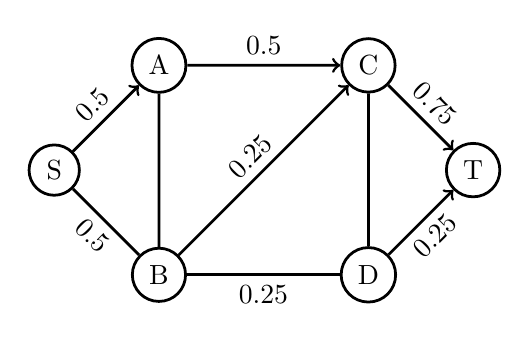
\begin{tikzpicture}[scale=1.33]
\begin{scope}[line width=1pt]
\node[circle,draw] (S) at (0.0,1.0) {S};
\node[circle,draw] (T) at (4.0,1.0) {T};
\node[circle,draw] (A) at (1.0,2.0) {A};
\node[circle,draw] (B) at (1.0,0.0) {B};
\node[circle,draw] (C) at (3.0,2.0) {C};
\node[circle,draw] (D) at (3.0,0.0) {D};
\draw (S) --node[anchor=north,rotate=-45]{0.5} (B);
\draw (A) -- (B);
\draw (B) --node[anchor=north]{0.25} (D);
\draw (C) -- (D);
\draw[->] (S) --node[anchor=south,rotate=45]{0.5} (A);
\draw[->] (A) --node[anchor=south]{0.5} (C);
\draw[->] (B) --node[anchor=south,rotate=45]{0.25} (C);
\draw[->] (C) --node[anchor=south,rotate=-45]{0.75} (T);
\draw[->] (D) --node[anchor=north,rotate=45]{0.25} (T);
\end{scope}
\end{tikzpicture}
\end{center}
\caption{ECMP forwarding one unit of traffic from S to T leads to imbalanced traffic load.}\label{fig:badecmp}
\end{figure}

\figurename~\ref{fig:badecmp} shows an example that the parallel
paths according to ECMP are not disjoint and the traffic is imbalanced. We
assume each link in \figurename~\ref{fig:badecmp} has equal weight in the
shortest path computation. The arrows between nodes denotes the shortest path
tree toward T. When one unit of traffic is sent from S to T, the ECMP routing
logic will split the traffic to each link as shown in the figure. Here we can
see, the link CT is carrying three times more traffic than link DT, because at
each node ECMP splits traffic equally amongst all the valid next hops. To solve
this problem, optimized multipath \cite{ospfomp} and adaptive multipath
\cite{gzrr03} are proposed. They make use of the packet loss information to
split the traffic amongst different paths. In essense, the traffic load on a
path is adaptive to the level of congestion. However, we can see that, the same
problem can be solved easily by removing the path S-B-C-T, i.e. not to use all
the available multipaths but a subset of them.

How can we use a subset of available paths in multipath routing? An easy way is
to build the multipath using tunnels, such as the MPLS label switched paths. As
the OpenFlow architecture \cite{mabpprst08} getting popular, we can also make
use of the flexibility to pin point a path in OpenFlow switches or manipulating
their forwarding table to achieve the same goal. Therefore, the remaining
problem is that, how should we select the paths for multipath routing, so that
we can have a better load-balancing or equivalently, minimize the congestion.

In this paper, we attempt to solve the following problem: Given a topology, and
a set of flows, find the routes to deliver these flows with the constraint that
no any flow, defined as a traffic demand between a unique source-destination
pair, is routed over more than $k$ paths. For simplicity, we assume the traffic
of a flow is distributed evenly to all the viable paths. In other words, the
traffic distribution is \emph{not} adaptive to network congestions, so that we
avoid the issues of route change and their consequence of packet reordering.
The objective is to route efficiently, namely, to minimize the maximum link
utilization on the network.

This is similar to the multi-commodity flow problem \cite{pm04} but with
additional constraints on the traffic splitting. Afterwards, we will remove the
requirement of providing $k$ as a parameter, and to find the optimal number of
paths given the traffic matrix.

\section{The Algorithm}\label{sec:algo}

As the complexity in solving the multi-commodity flow problem for the optimal
solution is high, a heuristic algorithm is devised. The heuristic algorithm is
to find the multipaths individually between a pair of nodes. Since our goal is
to balance the network, i.e. minimize the maximum link utilization for the
given traffic matrix, we introduce a cost function to measure how good are the
paths. The outline of the algorithm is depicted in Algorithm \ref{alg:1}.

\begin{algorithm}
\caption{Algorithm to place routes on a network}\label{alg:1}
\KwData{Network topology $G=(V,E)$}
\KwData{Source-destination flows $F \subset V^2$}
\KwData{Estimated traffic matrix $\alpha_{st},\;\forall (s,t)\in F$}
\KwData{Maximum number of paths for a flow $k$}
Initialize link load account $\lambda_e :=0,\quad\forall e\in E$\;
\ForEach{$(s,t)\in F$ in random order}{\label{alg:mpathenum1}
  \tcc{Find the candidate paths from $s$ to $t$}
  $M$ := all valid paths joining $s$ to $t$\;\label{alg:pathfind}
  \tcc{Select $k$ paths}
  \For{$i:=1$ to $k$}{
    $p$ := the path among $M$ with the lowest path cost\;
    $\lambda_e$ increase by $\frac{1}{k}\alpha_{st}$ for all $e\in p$
  }
}
\end{algorithm}

The heuristic algorithm is a greedy algorithm that selects one path at a time,
assuming that we can minimize the overall maximum link utilization by
minimizing the path cost in every step. The algorithm takes a traffic matrix as
the input to provide estimate of the relative size of traffic between different
pairs of nodes. Whether the traffic matrix can be fulfilled in the network is
not a concern, but it may have influence on the cost function, for example, a
cost function that models the links as queues will find an unfulfillable
traffic matrix to yield an infinite cost. The idea of the algorithm is as
follows: We first initialize link load values $\lambda_e$ to zero. They serve
as the scoreboard for the amount of traffic assigned to the links. Then we
examine each pair of nodes in a random order, to select the $k$ best paths on
the network that connect them. A cost function returns a cost for every path
based on the current load on each link. The $k$ best paths are selected so that
they correspond to the lowest cost according to the current $\lambda_e$. Once
the paths are selected, all the corresponding $\lambda_e$ are increased by
$\alpha_{st}/k$, where $\alpha_{st}$ is the amount of traffic from $s$ to $t$,
to reflect that these links are carrying additional traffic. For simplicity, we
assume an even distribution of load to these $k$ paths. This can serve as the
lower bound on the performance if adaptive multipath routing is being used. At
the end of the algorithm, $\lambda_e$ reflects the resulting utilization as the
multipaths are selected accordingly.

The selection of the best $k$ paths (the inner loop in the algorithm) to
connect $s$ to $t$ is as follows: If there are no more than $k$ valid paths
available, all of them are chosen. The valid path is the one without loop, and
fulfilling other constraints such as path length. More detail on the validity
are addressed in later paragraphs. In case there are more than $k$ valid paths,
the best path among all the candidate paths are chosen according to a path cost
function. This function is to evaluate the resulting utilization if this path
is used. The evaluation is based on the current link load account $\lambda_e$, the
links' capacities, and the estimated offered load $\alpha_{st}$ for the flow in
consideration. Once the best path is found, the corresponding link load is
increased by $\alpha_{st}/k$ to reflect the fact that this path is going to
carry $\frac{1}{k}$ of the traffic as we are going to evenly distribute the
traffic among the $k$ paths selected. This process is repeated for $k$ times to
select the $k$ best paths from the pool of candidates.

Note that, because the link load account is to reflect the estimated traffic
amount, there is no upper limit for $\lambda_e$ as long as it is non-negative.
Therefore, $\lambda_e$ could be greater than the link capacity, as a result of
traffic demand overloaded the network capacity. The algorithm here does not
prevent this to happen, but only to optimize for better load balancing.

The path cost function is the core of the heuristic algorithm. It quantizes the
preference of a path over another. One way to set up such cost function is to
take the sum of the relative load of all the links. Assume the link capacities
are denoted by $\mu_e$, the cost function for a path $p$ to carry $1/k$ of the
traffic from $s$ to $t$ is therefore, 

\begin{align}
\chi(p) = \sum_{e\in p} \frac{\lambda_e + \alpha_{st}/k}{\mu_e}
\label{sumfunction}
\end{align}

The fraction reflects the load on link $e$ when this path is selected and
carries $\frac{1}{k}$ of the traffic from $s$ to $t$. The summation accounts
for the end-to-end congestions, so that it prefers a shortest path if
everythings are equal. Another way to set up a cost function is to take the
maximum load instead of the summation, so that it is indifferent to the path
length but avoid to raise the maximum link load on the network.

\begin{align}
\chi(p) = \max_{e\in p} \frac{\lambda_e + \alpha_{st}/k}{\mu_e}
\label{maxfunction}
\end{align}

We could also have the cost function in between of equations \eqref{sumfunction}
and \eqref{maxfunction}, i.e.

\begin{align}
\chi(p) = \sum_{e\in p} f\big(\frac{\lambda_e + \alpha_{st}/k}{\mu_e}\big),
\label{midfunction}
\end{align}
where $f(x)$ is a monotonically increasing convex function, such as $f(x)=x^2$
or $f(x)=e^x$.

In case the cost function reports equal for several paths, we use the path
length as the tie-breaker. When the paths are of equal length, we randomly
choose among them.

In line \ref{alg:pathfind} of the algorithm, we enumerate the valid paths that
joins $s$ to $t$. We can use a modified Eppstein's algorithm to do this, as
follows.

\begin{algorithm}
\caption{Path finding algorithm}
Run Bellman-Ford algorithm to find the shortest path from any node to $t$,
let $d(v)$ denotes the shortest path distance from $v$ to $t$\;
$T$ := the tree composed of the the shortest paths to $t$\;
$S$ := the set of links not in $T$, a.k.a. sidetrack links\;
\ForEach{$e\in S$}{
  \tcc{Assume $e$ is a directed edge joining $u$ to $v$}
  $c(e)$ := $d(v) - d(u) + w(e)$, where $w(e)$ is the length of link $e$
}
Start with an empty priority queue $Q$\;
$Q$.push($\emptyset$ with priority 0)\;
\While{$Q$ not empty}{
  $\sigma$ := $Q$.pop()\;
  Output the shortest path from $s$ to $t$ according to $T$ and $\sigma$\;
  \ForEach{$e\in S-\sigma$}{
    $\sigma'$ := $\sigma \cup \{e\}$\;
    \If{$\sigma'$ represents a valid path}{
      $Q$.push($\sigma'$ with priority $\sum_{e\in\sigma'} c(e)$)\;
    }
  }
}
\end{algorithm}

The core of the Eppstein's algorithm is the shortest path tree $T$ terminated
at $t$ as given by the Bellman-Ford algorithm. The tree is a directed graph
such that each arc is pointed to $t$. We can find the shortest path from any
node $v$ to $t$ by traversing along the arc in this tree. Any loop-free path
other than the shortest path according to this tree $T$ can be represented by a
set of \emph{sidetrack} edges. The sidetrack edges are directed edges. They are
the edges that are traversed in a path but not included in $T$. When a set of
sidetrack edges are given, the path from $s$ to $t$ is constructed as follows:
We start from node $s$ on the network, and traverse the edges until we reach
$t$. At every node, the edge to traverse is determined uniquely by first
looking for any edge that is included in the set of sidetrack edges. If none
are found, then we follow the edge on the shortest path tree $T$. Therefore, a
well-formed set of sidetrack edges shall not contain more than one edge
emerging from the same node. Moreover, the path constructed in this way shall
exhaust all the provided sidetrack edges to make this set of sidetrack edges
well-formed. Thus, for any loop-free path, there is a corresponding set of
sidetrack edges, but not vice versa.

The latter half of the path finding algorithm is crucial to enumerate the paths
in ascending order of path length. The quantity $c(e)$ represents the penalty
of using a sidetrack edge $e$ in terms of the length of resulted path, $c(e)
\ge 0$ guaranteed. Therefore, for a well-formed set of sidetrack edges,
$\sigma$, the length of the corresponding path $p$ is \[
\ell(p) = d(s) + \sum_{e\in\sigma} c(e) \]
where $d(s)$ is the shortest path distance from $s$ to $t$ and the summation is
the total additional length imposed by traversing the sidetracked edges.
Therefore, for any set $\sigma'$ that is a superset of $\sigma$, the
corresponding path of the former must be no shorter than that of the latter.
Making use of this property, the while-loop in the above algorithm use a
priority queue to enumerate the paths in ascending order of lengths. And
because of this, we can terminate the path-finding algorithm prematurely if we
impose a constraint on the length of paths to be found. For example, we can
limit to our search to only shortest paths (i.e. paths of the length equal to
$d(s)$) by skipping the set of sidetrack edges $\sigma'$ whenever
$\sum_{e\in\sigma'} c(e) > 0$ is found.

\section{Limitations of the Algorithm}

The algoritm to find the $k$ paths for all the source-destination pairs is
presented in the previous section. The algorithm does not try to find the
global optimal but instead, it is a heuristic algorithm to approximate the
solution.

Because the heusitic algorithm searches the paths in a greedy manner, there are
three limitations:

\begin{itemize}
\item Because the paths for each source-destination pair is computed
individually, no coordination can be done to strategically use different paths
for different source-destination pairs to avoid conflicts, which can incur
congestion.
\item The way to find $k$ paths for a particular source-destination pair is to
find the paths one by one according to the updated path cost. In this way,
similarly, we cannot coordinate the selection between these $k$ paths.
\item The algorithm intended to find $k$ paths for a source-destination pair
whenever it is possible. However, for the objective of minimizing the maximum
link load, the best solution may not be utilzing all the $k$ paths.
\end{itemize}

Moreover, the algorithm is based on the assumptions that,
\begin{itemize}
\item Any arbitrary loop-free path can be used to forward traffic; and
\item The traffic demand is known a priori.
\end{itemize}
We do not see these as major hurdles. The former can be readily achieved by
setting up end-to-end paths, such as MPLS LSP. The latter is also a reasonable
assumption and we can merely estimate the traffic matrix by statistics of
historical usage data.

\section{Result}

Two sets of evaluations is done on this algorithm, to compare its performance
against the standard ECMP. The first evaluation is to compare the traffic load
on each links as a result of even distribution according to ECMP, and according
to the path-finding of the algorithm.

\subsection{Fluid traffic demand}

We first assume the traffic demand provided is fluid demand. In other words, we
can split the traffic evenly across a number of paths. The traffic distribution
as depicted in page 1 is the result of fluid traffic splitting according to
ECMP. We compare the load distribution according to ECMP against the case of
$k$ paths being found by our algorithm. We run the algorithm twice to find two
set of paths: Firstly the paths are limited to shortest path only, therefore
they are a subset of the paths being used by ECMP (denoted by `k-short').
Secondly we do not impose any constrain on the paths besides they have to be
loop free (denoted by `k-free'). Therefore, they may be of longer length. In
the following, we fixed $k=4$ in our evaluations and defined the path length as
the hop count.

\begin{figure}
\centering\includegraphics[width=0.8\columnwidth]{cost-max/ft-4.all.full.pdf}
\caption{Fat-tree network of degree 4}
\end{figure}

In figure 1, we evaluate the different way of routing traffic by a fat-tree
topology of degree 4. The horizonal axis represents the links in ascending
order of load. The vertical axis represents the load to a link, in some
arbitrary unit. The traffic matrix used here assumes all the host in the
network send a unit traffic to every other hosts. Because of the highly regular
topology, the ECMP performed the best in terms of both load balancing and
minimizing the maximum link load across the network. Interestingly, the
$k$-path algorithms performs differently depend on whether the
shortest-path-only constraint is imposed. When we limit our paths to only
shortest-path, the performance is not as good as ECMP but close enough. The
difference from ECMP is due to the heuristic nature of the algorithm, namely,
it does not coordinate the path selection between the source-destination pairs.

In case the path selection is free from the path length constraints, we found
that it performs badly. One can see from the figure that, the heaviest loaded
link is way more loaded than the case in ECMP. Moreover, some links are under
utilized. These are resulted from the inefficiency of the heuristic algorithm.
Furthermore, the total area under the curve is also larger in this case than
the other two, reflecting the fact that the paths selected are lengthier in
general.

\begin{figure}
\centering\includegraphics[width=0.8\columnwidth]{cost-max/att.all.full.pdf}
\caption{Irregular topology (AT\&T)}
\end{figure}

Besides the regular topologies like fat-tree, we also evaluated on irregular
topologies. Figure 2 shows one of the results. This is a typical result from an
irregular network: The curves of ECMP and k-short are not narrow and flat, but
instead, crossing a broad spectrum of link loads. This is resulted from the
property of the irregular topologies that, certain links are `hot links' of the
network that are more popular, so that they carried significantly heavier load
than others. The curves of ECMP and k-short are almost coincide. Therefore,
k-short performed as good as ECMP. Surprisingly, unlike the case in fat-tree,
the curve of k-free shows a more balanced link load and lower maximum link
utilization (compare the rightmost end of the curves). This is because, as hot
links are present in the topology, lifting the shortest-path constraint to path
selection allows us to detour around those hot spots, and hence lowered its
load. The links at the rightmost end of the curves correspond to those hot
links. We can observe a significant decrease in the load in k-free compared to
the other two.

\begin{figure}
\centering\includegraphics[width=0.8\columnwidth]{cost-max/level3.all.full.pdf}
\caption{Irregular topology (Level-3)}
\end{figure}

Such result in the irregular topology as mentioned above is particular to the
particular toplogy. While we observe similar result in many topologies in
Rocketfuel, we also found a few topology that shows no significant difference
between the different ways of multipath forwarding. Figure 3 is such an
example. We can see that the curves of the three methods of placing load are
more or less identical. This is because the network in concern does not show
enough path diversity. In other words, the limitation of the topology makes the
difference between the different methods unobservable.

Among these figures shown, we can find that
\begin{itemize}
\item ECMP and k-short performed roughly as good as each other; and
\item k-path is better then ECMP and k-short in irregular topologies where
there are a few hot spot links. This also supports the claim that ECMP is not
always optimal.
\end{itemize}
Therefore, by using k-short, it is possible to use fewer number of forwarding
path for a source-destination pair than ECMP, but without sacrificing the
balance of load as provided by ECMP.

The path cost function used in producing the above figures are
\eqref{maxfunction}. We also repeated the experiment with the other three cost
functions mentioned in section 3. Those result is consistent with the above
claims, but slightly different in the magnitude of the link loads. One can
compare figure 4, which is using \eqref{sumfunction} as the cost function,
against figure 2. Whereas the other two curves are almost the same, the curve
corresponding to k-free gives a smaller maximum link load in figure 4.

\begin{figure}
\centering\includegraphics[width=0.8\columnwidth]{cost-sum/att.all.full.pdf}
\caption{Irregular topology (AT\&T), using \eqref{sumfunction} as cost function}
\end{figure}

\subsection{Dynamic traffic distribution}

Another set of evaluation is performed assuming we have to place individual
flows on demand. 

This evaluation is performed as follows: Assume we have the topology and
traffic matrix as before, we can then find the forwarding paths for different
source-destination pairs according to the algorithm. Then, we read the flow
descriptions and place them into the network. The description of one flow
provides the information about the flow's source and destination node, the size
(in term of traffic rate of data), the time of arrival, and its holding time.
We assume it is a CBR flows of predetermined holding time for simplicity. A
flow is placed into the network one at a time. Each flow uses one path, even if
the network provided enough path diversity. This is to simulate the fact that,
we usually keep a flow into only one path to avoid packet reordering. The path
selection for a particular flow is random. Adaptive placement of flows
according to the real-time load can be a future extension. When a flow is
placed to a path, all the links correspond to this path would have their load
increased. We keep track on the load of each link at any time.

\begin{figure}
\centering\includegraphics[width=0.48\columnwidth]{ft-4.TrimEcmp.png}
\centering\includegraphics[width=0.48\columnwidth]{ft-4.SimuEcmp.png}
\caption{Fat-tree topology of degree 4, link load vs time}
\end{figure}

Figure 5 shows the result from the evaluation using dynamic traffic. The
topology is consideration is a fat-tree topology built with 8-port switches.
The traffic matrix used is same as the one in the previous evaluation, namely,
each pair of source-destination nodes has one unit of traffic. The flow dynamic
used is to have Poisson arrival and exponential holding time, with a flow size
draw randomly from a uniform distribution between 0 and 1. The arrival of flows
lasts from time 0 to 100. The horizontal axis in figure 5 represents the time,
the vertical axis is the size of link load. Each link in the topology is
represented by one continuous curve, showing its link load at any given time.

The two plots in figure 5 compares the link load when ECMP is used against the
k-path and k-short schemes. The topology contains 512 unidirectional links,
therefore the each plot shows 512 curves of the same color, corresponding to
the different way of multipath forwarding. On the left plot, we see that the
two `walls' of curves corresponding to ECMP and k-short are overlapping almost
perfectly. This means the k-short perform as good as ECMP from the point of
view of overall link load across the network. On the right plot, however, the
`wall' correspond to k-path is bigger than that of ECMP: Which the red area
surrounded the green area entirely. This tells that k-path has a worse
performance than ECMP, not only it is less balanced (i.e. wider in the plot),
but also the heaviest link carries more traffic than the ECMP counterpart (by
observing the top border of the colored area). Note, the green area in the two
plots, which correspond to the case of ECMP, are identical.

\begin{figure}[h]
\centering\includegraphics[width=0.48\columnwidth]{att.TrimEcmp.png}
\centering\includegraphics[width=0.48\columnwidth]{att.SimuEcmp.png}
\caption{Irregular topology (AT\&T), link load vs time}
\end{figure}

Similarly, figure 6 shows the case on an irregular topology same as the one in
figure 2. On the left plot, we see the same result as in figure 5. The
performance of ECMP and k-short are roughly identical. On the right plot,
however, we can see an observable improvement of k-path over ECMP by comparing
the topmost curve of the two colors. This time, the k-path gives a more
balanced load than ECMP on this particular topology.

In summary, although we do not consider a flow can be splitted in this
evaluation, we see the conclusion the same here as in section 5.1, namely,
k-short is as good as ECMP is all scenarios tested, and k-path can perform
better in irregular topologies where there are a few hot-spot links, or perform
worse in highly regular topologies such as fat-tree.

\subsection{Effect on $k$}

We have also repeated the experiment with different values of $k$.

\begin{figure*}
\includegraphics[width=0.33\textwidth]{att.k=2.pdf}%
\includegraphics[width=0.33\textwidth]{cost-max/att.all.full.pdf}%
\includegraphics[width=0.33\textwidth]{att.k=8.pdf}
\caption{Irregular topology (AT\&T), with $k=2,4,8$ respectively from left to right}
\end{figure*}

Figure 7 shows the case for the typical irregular topology. Overall, there are
not much difference between the case of $k=2$, $k=4$, and $k=8$. Surely, ECMP
and k-short are mostly identical in all the three plots. The curves for k-path,
however, only shows a minor change. The load of the heaviest link according to
k-path decreased slightly as $k$ increases. This behaviour can be explained by
the property of the topology that a high degree of path diversity is not
available in many source-destination pairs. Therefore, even if we increase $k$,
the choice is not enlarged much. Moreover, even if more paths are available for
a source-destination pair, the paths are likely not mutually disjoint, which we
cannot reduce the load on those shared links by multipath routing.

\begin{figure*}
\includegraphics[width=0.33\textwidth]{ft-4.k=1.pdf}%
\includegraphics[width=0.33\textwidth]{ft-4.k=2.pdf}%
\includegraphics[width=0.33\textwidth]{cost-sum/ft-4.all.full.pdf}
\caption{Fat-tree topology, with $k=1,2,4$ respectively from left to right}
\end{figure*}

The counterpart for fat-tree topology is shown in figure 8. As we know from
section 5.1, k-path does not perform well in such topology due to the
inefficiency of the heuristic algorithm. However, we see a difference on
k-short as we increase the value of $k$. When $k=1$, we see that k-short
perform poorly. This is because we did not exploit the path diversity available
to balance the load. But as $k=2$ or above, the performance of k-short is close
to ECMP. Further increasing the value of $k$ only introduces marginal
improvement. This shows that, we do not need a lot of parallel paths to bring a
balanced load to a network. A small number of paths is sufficent. This also
endorses our claim that we do not need to use the extensive path diversity as
in ECMP to achieve a good load balancing.

\balance
\bibliographystyle{IEEEtran}
\bibliography{ecmp}

\label{docend}
\end{document}
